
\begin{table*}[tb]
\centering
\setlength{\tabcolsep}{5pt}
\renewcommand{\arraystretch}{1.15}
\caption{
Multi-objective search results for configurations from a BoTorch run on \llamaIIISmall.
% We report perplexity (↓) from the accuracy evaluator, end-to-end latency (seconds ↓), and area (\(\mu\text{m}^2\) ↓). 
We showcase four representative design points on the Pareto frontier with different perplexity (↓), latency (seconds ↓), area (\(\mu\text{m}^2\) ↓) trade-offs. 
The complete empirical attainment surfaces of the multi-objective search are in \Cref{fig:codesign_eas}.
\best{Best} results are highlighted. 
}
\label{tab:one_frontier}

\resizebox{\textwidth}{!}{%
\begin{tabular}{lccccccccccc}
\toprule
\multicolumn{9}{c}{Parameters} &
\multicolumn{3}{c}{Metrics} \\
\cmidrule(lr){1-9}
\cmidrule(lr){10-12}
\texttt{BLEN} & \texttt{MLEN} & \texttt{VLEN} &
\texttt{M\_LOAD} & \texttt{V\_LOAD} & \texttt{V\_WRITE} &
\texttt{ACT\_WIDTH} & \texttt{KV\_WIDTH} & \texttt{FP\_SETTING} &
Perplexity $\downarrow$ & Lat (s) $\downarrow$ & Area (\(\text{mm}^2\)) $\downarrow$ \\
\midrule
32 & 512  & 128 & 128 &  64 & 256 & MXFP\_E4M3 & MXFP\_E3M4 & FP\_E4M7 &  6.70 & 0.137 & 137.6 \\
32 & 1024 & 1024& 256 & 256 & 128 & MXINT\_8   & MXINT\_4   & FP\_E3M2 &  6.76 & \best{0.116} & 203.4 \\
8  & 128  &  32 & 128 &   8 & 256 & MXFP\_E3M4 & MXFP\_E3M4 & FP\_E5M6 &  \best{6.54} & 0.166 & 26.45 \\
16 & 128  &  16 &   4 &  16 &  64 & MXINT\_8   & MXFP\_E4M3 & FP\_E3M2 &  6.60 & 0.174 & \best{23.64} \\
\bottomrule
\end{tabular}%
}
\vspace{-10pt}
\end{table*}

\section{Evaluation}


\subsection{Experiment Setup}
\paragraph{Models and Datasets} 

We evaluate our quantization framework on popular open-source LLMs, namely LLaMA-2~\cite{llama2} and LLaMA-3~\cite{llama3}, as well as MoE~\cite{MoE} (e.g.~GPT-OSS) and Qwen3 models. Quantization performance is measured in terms of perplexity on the WikiText-2 dataset~\cite{wikitext2}.

The entire quantization process requires approximately 2–20 GPU hours on NVIDIA H100 GPUs. 

\paragraph{Quantization Baselines} 
We compare against several SoTA quantization methods, including software-based approaches targeting GPUs such as GPTQ~\cite{frantar2022gptq}, OmniQuant~\cite{shao2023omniquant}, and QuaRoT~\cite{QuaRot}, as well as approaches used on hardware accelerators such as Atom~\cite{zhao2024atom} and MicroscopiQ~\cite{Microscopiq}.

\paragraph{Accelerator Implementation} PLENA is implemented in SystemVerilog RTL. We perform synthesis using the Synopsys Design Compiler with the 7\,nm OpenROAD predictive PDK~\cite{openroad}. This helps us to generate area and power estimates at a 1\,GHz clock frequency. 


\paragraph{Accelerator Baselines} Since our baselines—MicroscopiQ~\cite{Microscopiq}, FIGNA~\cite{FIGNA}, and Olive~\cite{guo2023olive}—are not fully open-sourced or cannot be evaluated under a consistent technology node and toolchain, we re-implemented their core components and integrated them into the PLENA system for a fair inference performance comparison. Additionally, DeepScale~\cite{DeepScale} is used for overall system performance estimation, scaling all designs to the 7\,nm process. Detailed area and power of the core units are evaluated using our own implementations.

\paragraph{Inference Process}
Instead of comparing only with prior accelerator designs, we also evaluate PLENA against high-performance commercial compute platforms, including GPUs (A100 80GB and H100 80GB) and TPUs (v6e-8), to provide a fair and practical comparison. The GPU experiments are conducted in an environment with Ubuntu~22.04, CUDA~12.8, Python~3.11, PyTorch~2.8.0, and vLLM~0.10 V1. The TPU experiments are conducted in an environment with v2-alpha-tpuv6e software.

\subsection{Balancing Area, Latency and Perplexity via Co-design}

%-----------------------------------
\label{subsec:co_design_exp}

This subsection shows the results of our design space exploration experiments. Figure~\ref{fig:codesign_eas} shows the Empirical Attainment Surfaces (EAS) for the Pareto fronts found when optimizing with \llamaTiny and \llamaIIISmall. EAS is a visualization approach well-suited for conveying the uncertainty of the Pareto fronts from multiple runs with different random seeds~\cite{knowles2005eas, fonseca2011eas}. Existing tools support visual analysis for two objectives~\cite{watanabe2023eas}, hence we plot EAS for accuracy and latency first. Figure~\ref{fig:codesign_eas} shows that active learning with BoTorch sampler achieves a significantly better tradeoff between latency and perplexity than naive randomized sampling. Tree-Structured Parzen Estimator (TPE) shows more modest gains when optimizing with \llamaTiny compared to using BoTorch sampler, thus we focus on the latter for experiments with \llamaIIISmall.

\begin{figure}[!t]
  \centering
  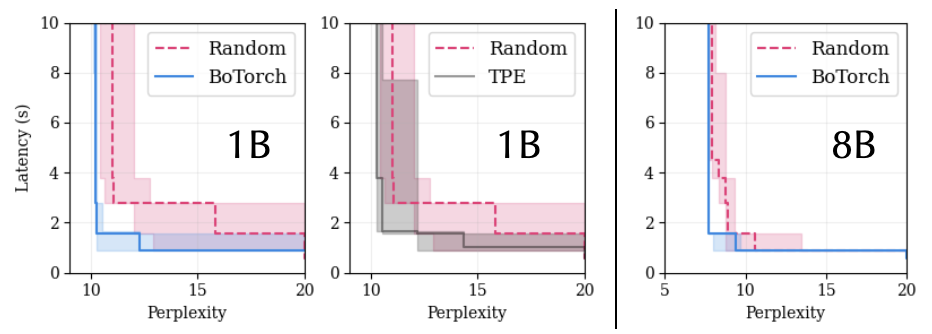
\includegraphics[width=0.485\textwidth]{Figures/co-design-1b-and-8b.png}
\caption{Empirical Attainment Surfaces for latency ($\downarrow$) and perplexity ($\downarrow$) objectives across multiple seeds, evaluated with \llamaTiny and \llamaIIISmall over the co-design space shown in \Cref{tab:design_space}.
For the 1B model, we run 9 seeds with 50 trials, comparing BoTorch and TPE methods against Random sampling. 
For the 8B model, we run 5 seeds with 50 trials, comparing BoTorch against Random. 
Shaded regions show the 25\% and 75\% attainment bands across seeds.}
  \label{fig:codesign_eas}
  \vspace{-15pt}
\end{figure}

In \Cref{tab:one_frontier}, we show our co-design results generated from multi-objective optimization runs. These runs can yield designs featuring various trade-offs along the Pareto frontier, with some naturally incorporating multi-precision and multi-arithmetic elements. The PLENA system facilitates such exploration, thanks to its comprehensive simulation and RTL support for these arithmetic types and precision levels.

 

\subsection{Preserving MX Perplexity via Clipping \& Rotation}
\label{subsec:quantization_experiments}

\paragraph{Main Results}
\begin{table}[t]
    \centering
\caption{\wiki perplexity (\textbf{$\downarrow$}) under GEMM-only emulation (nonlinear ops in full precision) for \llamafamily. 
% Results for GPTQ, AWQ, OmniQuant, and Atom are taken from MicroScopiQ; QuaRot numbers are from the paper or reproduced when not reported. 
W/A/KV denote bit widths for weights, activations, and KV cache. Results marked with $^*$ are reproduced from released code.}

\resizebox{1.0\linewidth}{!}{
    \begin{tabular}{lcccccc}
    \toprule
    &   & \multicolumn{3}{c}{\textbf{LLaMA-2} \cite{llama2}} & \multicolumn{2}{c}{\textbf{LLaMA-3} \cite{llama3}} \\
    \cmidrule(lr){3-5}
    \cmidrule(lr){6-7}
    \textbf{Method} & \textbf{W/A/KV}  & \textbf{7B} & \textbf{13B} & \textbf{70B} & \textbf{8B} & \textbf{70B} \\
    \midrule
    Baseline & 16/16/16 & 5.47 & 4.83 & 3.31 & 6.13 & 2.85 \\
    \midrule
    GPTQ \cite{frantar2022gptq} & 4/16/16 & 6.23 & 5.58 & 4.28 & 8.12 & 3.75 \\
    AWQ \cite{lin2024awq} & 4/16/16 & 5.82 & 5.19 & 4.08 & 7.96 & 3.58 \\
    OmniQuant \cite{shao2023omniquant} & 4/16/16 & 5.74 & 5.02 & 3.47 & 7.09 & 3.46 \\
    MicroScopiQ \cite{Microscopiq} & 4/16/16 & 5.65 & 5.02 & 3.42 & 6.89 & \best{3.25} \\
    QuaRot \cite{QuaRot} & 4/16/16 & \best{5.60} & 5.00 &  3.41& 6.52$^*$ &  3.53$^*$ \\
    \textbf{PLENA (MXFP)} & 4/16/16 & 7.09 & 5.91 & - & 11.95 & - \\
    \textbf{PLENA (ours)} & 4/16/16 & 5.61 & \best{4.97} & \best{3.41}& \best{6.45} & 3.59 \\
    \midrule
    OmniQuant \cite{shao2023omniquant} & 4/4/16 & 11.47 & 8.32 & 5.41 & 10.21 & 5.30 \\
    SmoothQuant \cite{xiao2023smoothquant} & 4/4/16 & 20.47 & 15.63 & 17.62 & 29.54 & 19.32 \\
    Atom \cite{zhao2024atom} &  4/4/16 & 6.16 & 6.12 & 5.20 & 8.12 & 4.69 \\
    MicroScopiQ \cite{Microscopiq} &  4/4/16 & 6.11 & 5.57 & 4.48 & 8.12 & 4.65 \\
    QuaRot \cite{QuaRot}& 4/4/16 & 6.02$^*$  & 5.36$^*$ & 3.78& 8.00$^*$& 6.33$^*$ \\
    M-ANT \cite{hu2025mant}& 4/4/16 & 5.92  & 5.24 & - & - & - \\
    \textbf{PLENA (MXFP)} & 4/4/16 & 15.89 & 10.30 & - & 91.71 & - \\
    \textbf{PLENA (ours)} &  4/4/16 & \best{5.69} & \best{5.03} & \best{3.59}& \best{6.76} & \best{4.51} \\
    \midrule
    QuaRot \cite{QuaRot} & 4/4/4 & 6.10 & 5.40 & 3.79&  8.16 & 6.66 \\
    QuaRot-128G \cite{QuaRot}& 4/4/4 & 5.93& 5.26 & \best{3.61} & 7.36&  5.51 \\
    \textbf{PLENA (MXFP)} & 4/4/4 & 67.35 & 27.44 & - & 256.22 & - \\
    \textbf{PLENA (ours)} &  4/4/4 & \best{5.89} & \best{5.18} & 3.62 & \best{7.22} & \best{4.77} \\
    \bottomrule
    \end{tabular}}
    \label{tab:llm_results}
    % \vspace{-10pt}
    % \parbox{1.0\linewidth}{\small\emph{Note: Results marked with $^*$ are reproduced from the authors’ released code. 
    % Specifically, for the QuaRot 4/4/16 configuration, we follow the experimental setup described in their paper, where activations are symmetric-quantized with a clipping ratio of 0.9.}}
\end{table}



\begin{table}[t]
\centering
\caption{Ablation study of quantization techniques and their impact on microscaling data formats, evaluated across all 9 GEMMs in \llamaIIISmall. Results are reported on \wiki{} perplexity. GPTQ is used for clipping: $\mathrm{Err}_{y}$ denotes output-norm clipping; $\mathrm{Err}_{w}$ denotes weight-norm clipping.}
\label{tab:ablation}

\resizebox{\linewidth}{!}{

\begin{tabular}{lrlr}
\toprule
\textbf{Method} & \multicolumn{1}{l}{\textbf{PPL\textbf{$\downarrow$}}} & \textbf{Method} & \multicolumn{1}{l}{\textbf{PPL\textbf{$\downarrow$}}} \\
\cmidrule(lr){1-2}
\cmidrule(lr){3-4}
\textbf{Baseline FP16} & 6.13 & \multicolumn{2}{l}{\textbf{ACT and KV Only}} \\
\cmidrule(lr){1-2}
\multicolumn{2}{l}{\textbf{Weight Only}} & MXFP4 & 29.75 \\
MXINT + RTN & 6.83 & MXINT4 & 7.24 \\
MXFP + RTN & 11.94 & MXFP4 + Selective Rotate & 14.50 \\
MXINT4 + Rotation & 6.98 & MXINT4 + Selective Rotate & \best{7.05} \\
\cmidrule(lr){3-4}
MXFP4 + Rotation & 13.71 & \multicolumn{2}{l}{\textbf{MXINT Full System}} \\
MXINT4 + $\mathrm{Err}_{w}$ Clip & 6.53 & RTN & 8.28 \\
MXINT4 + $\mathrm{Err}_{y}$ Clip & \best{6.45} & $\mathrm{Err}_{y}$ Clip & 7.60 \\
\multicolumn{2}{l}{\textbf{}} & $\mathrm{Err}_{y}$ Clip +Selective Rotation & \best{7.22} \\
\bottomrule
\end{tabular}
}
\vspace{-13pt}
\end{table}


\begin{table}[t]
    \centering
    \footnotesize
    \setlength{\tabcolsep}{3.5pt}
    \caption{Zero-shot downstream task accuracy of LLaMA-3 models with 4-bit weight, activation, and KV quantization, evaluated on PIQA (PQ), WinoGrande (WG), HellaSwag (HS), Arc-Easy (A-e), Arc-Challenge (A-c), and LAMBADA (LA).}
    \begin{tabular}{l|cccccc|c}
        \toprule
        \textbf{Method} & \textbf{PQ} & \textbf{WG} & \textbf{HS} & \textbf{A-e} & \textbf{A-c} & \textbf{LA} & \textbf{Avg.} \\
        \midrule
        \multicolumn{8}{l}{\textit{LLaMA-3-8B}} \\
        \quad FP16                 & 80.74 & 72.77 & 79.06 & 77.82 & 53.33 & 75.63 & 73.22 \\
        \quad QuaRot~\cite{QuaRot} & 75.14 & 65.82 & 72.94 & 68.01 & 43.34 & 65.81 & 65.18 \\
        \quad \textbf{PLENA (ours)}&79.00  & 71.90 & 76.07 & 74.71 &  48.21 & 72.44 & 70.39 \\
        \midrule
        \multicolumn{8}{l}{\textit{LLaMA-3-70B}} \\
        \quad   FP16   & 84.66 & 80.51 & 84.89 & 85.86 & 64.25 & 79.47 & 79.94 \\
        \quad  QuaRot & 78.07 & 69.30 & 77.33 & 73.44 & 47.53 & 69.57 & 69.21 \\
        \quad  \textbf{PLENA (ours)} &   82.48 &  77.51 &  83.47  & 78.54   &  57.17   &  78.05   &   76.20   \\
        \bottomrule
    \end{tabular}
    \label{tab:zero_shot_combined}
\end{table}



\begin{table}[t]
\centering
\caption{Evaluation of long-context and agentic workloads across code generation (HumanEval~\cite{chen2021codex}), mathematical reasoning (GSM8K~\cite{cobbe2021training}), and function-calling (BFCL-Web Search Base~\cite{patil2025berkeley}) benchmarks. W/A/KV denotes bit widths for weights, activations, and KV cache.}
\label{tab:long_context_agentic}
\begin{tabular}{lc ccc}
    \toprule
    \textbf{Model / Method} & \textbf{W/A/KV} & \textbf{HumanEval} & \textbf{GSM8K} & \textbf{BFCL-W} \\
     & & pass@1 $\uparrow$ & EM $\uparrow$ & Acc $\uparrow$ \\
    % \midrule
    % \multicolumn{5}{l}{\textit{Qwen3-8B}} \\
    % \quad Baseline              & 16/16/16 & 84.8 & 90.9 & 5.0 \\
    % \quad \textbf{PLENA (ours)} & 4/4/4    & 78.7   & --   & -- \\
    \midrule
    % \multicolumn{5}{l}{\textit{Qwen3-32B}} \\
    \quad Baseline              & 16/16/16 & 89.6 & 97.85 & 27.0 \\
    \quad \textbf{PLENA (ours)} & 4/4/4    & 84.1   & 97.85  & 24.0 \\
    \bottomrule
\end{tabular}
\vspace{-10pt}
\end{table}

\begin{table}[t]
\centering
\caption{Ablation study of quantization techniqeus on Qwen3 model across HumanEval, GSM8K, and BFCL-Web Search Base. $\mathrm{Err}_{y}$ denotes output-norm clipping. Qwen3-8B on HumanEval and GSM8K, Qwen3-32B on BFCL-Web Search Base. Results for HumanEval and GSM8K use Qwen3-8B; results for BFCL-Web Search Base use Qwen3-32B, as its higher baseline accuracy better isolates the effect of quantization.}
\label{tab:ablation_new}
\resizebox{\linewidth}{!}{
\begin{tabular}{l ccc}
    \toprule
    \textbf{Configuration} & \textbf{HumanEval} & \textbf{GSM8K} & \textbf{BFCL-W} \\
     & pass@1 $\uparrow$ & EM $\uparrow$ & Acc $\uparrow$ \\
    \midrule
    Baseline (FP16) & 84.8 & 90.9 & 27 \\
    \midrule
    W-only INT4 (RTN)      & 82.9 & 88.7 & 22 \\
    + ACT \& KV INT4       & 72.0 & 74.4 & 15 \\
    + GPTQ                 & 73.2 & 87.7 & 24 \\
    + $\mathrm{Err}_{y}$ Clip & 74.4 & 88.6 & 24 \\
    + Selective Rotation   & \best{78.7} & \best{88.8} & \best{24} \\
    \bottomrule
\end{tabular}}
\vspace{-10pt}
\end{table}

% \begin{table}[t]

% \centering
% \caption{Ablation study of quantization techniques and their impact on microscaling data formats, evaluated across all 9 GEMMs in \llamaIIISmall. Results are reported on \wiki{} perplexity, with ablations on (i) weights-only quantization, (ii) activation and KV-cache–only quantization, and (iii) full-system 4-bit quantization. GPTQ is used for all clipping methods: $\mathrm{Err}_{y}$ Clip denotes our output-norm–guided clipping search, while $\mathrm{Err}_{w}$ Clip denotes weight-norm–based clipping.}

% \label{tab:ablation}

% \begin{tabular}{ll|c}

% \toprule
% \textbf{Method} & \textbf{PPL\textbf{\best{$\downarrow$}}} \\
% \midrule
% \textbf{Baseline FP16} & 6.13 \\
% \midrule

% \multicolumn{2}{l}{\textbf{Weight Only}} \\
% MXINT + RTN & 6.83 \\
% MXFP  + RTN  & 11.94 \\
% MXINT4 + Rotation & 6.98 \\
% MXFP4 + Rotation & 13.71 \\
% MXINT4 + $\mathrm{Err}_{w}$ Clip & 6.53 \\
% MXINT4 + $\mathrm{Err}_{y}$ Clip & 6.45 \\

% % MXINT (8 / 6 / 4) & 6.14 / 6.19 /6.83 \\
% % MXINT4 + Err$_w$ Clip & 6.78 \\
% % MXFP6 (E1M4 / E2M5) & 6.33 / 6.15 \\
% % MXFP4 (E1M2 / E2M1) 
% %   & 11.95 / 3247.40 \\

% % MXFP4 (E1M2 / E2M1) + QuaRot 
% %   & 13.71 / 5377.72 \\

% % MXINT4 + QuaRot & 6.98 \\
% \midrule
% \multicolumn{2}{l}{\textbf{ACT and KV Only}} \\
% MXFP4 & 29.75 \\
% MXINT4 & 7.24 \\
% % MXFP4 + Rotation & 14.50 \\
% % MXINT4 + Rotation & nan \\
% MXFP4 + Selective Rotate & 14.50 \\
% MXINT4 + Selective Rotate & 7.05 \\
% \midrule
% \multicolumn{2}{l}{\textbf{MXINT Full System}} \\

% % $\mathrm{Err}_{w}$ Clip & 8.52  \\
% RTN & 8.28 \\
% $\mathrm{Err}_{y}$ Clip & 7.60  \\
% $\mathrm{Err}_{y}$ Clip +Selective Rotation& 7.22 \\
% % MXFP (E2M5 / E1M4) & 6.15 / 6.20 \\
% % MXINT (8 / 6) & 6.14 / 6.19 \\
% % \midrule
% % \multicolumn{2}{l}{\textbf{RTN (KV Only)}} \\
% % MXFP (E1M6 / E1M4) & 6.14 / 6.20 \\
% % MXINT (8 / 6) & 6.14 / 6.15 \\
% % \midrule

% % \multicolumn{2}{l}{\textbf{RTN + QuaRot (Weights Only)}} \\
% % MXFP4 (E1M2 / E2M1) & 13.71 / 5377.72 \\
% % MXINT4 & 6.9783 \\
% % \midrule

% % \multicolumn{2}{l}{\textbf{GPTQ (Weights Only)}} \\
% % INT4 & 8.12 \ \\
% % MXFP4 E1M2 & 8.19 \ \\
% % MXINT4 & 6.65 \ \\
% % MXINT4 + ($\mathrm{Err}_{\textbf{w}}$ Clip / $\mathrm{Err}_{\textbf{y}}$ Clip) & 6.53 / 6.45  \\
% % % MXINT4 + $\mathrm{Err}_{\textbf{y}}$ Clip & 6.45\\
% % \midrule
% % \multicolumn{2}{l}{\textbf{Full Model}} \\

% % W8A8KV8  \\
% % \midrule
% % MXINT4 + $\mathrm{Err}_{w}$ Clip & 8.52 \\
% % MXINT4 + $\mathrm{Err}_{y}$ Clip & \multirow{2}{*}{7.60} \\

% % MXINT4 + $\mathrm{Err}_{y}$ Clip & \multirow{2}{*}{7.2218} \\
% % + Selective Rotation  \\

% \bottomrule
% \end{tabular}
% \vspace{-10pt}
% \end{table}








% \subsection{Ablation Study on Quantization Methods}
% \begin{table}[h]
% \centering
% \caption{Ablation study on quantization techniques. Covering all 9 GEMMs in the \llamaIIISmall model. Quantization configured with W\_MXINT4, A\_MXINT4, KV\_MXINT4 with block size 16. }
% \begin{tabular}{l|c}
% \toprule
% \textbf{Method} & \textbf{ Perplexity (lower is better)} \\
% \midrule
% \textbf{Baseline FP16} & 6.14 \\
% \midrule
% RTN & 8.2763($2.3793\uparrow$) \\
% RTN + $\mathrm{Err}_{w}$ Clip &  8.1948($0.0815\downarrow$) \\
% GPTQ + $\mathrm{Err}_{w}$ Clip & 8.5193  ($0.3245\uparrow$) \\
% GPTQ + $\mathrm{Err}_{y}$ Clip & 7.6026 ($0.9167\downarrow$) \\
% \midrule
% GPTQ + $\mathrm{Err}_{y}$ Clip & \multirow{2}{*}{7.2218($0.3808\downarrow$)} \\
% + Selective Rotation  \\

% \bottomrule
% \end{tabular}
% \label{tab:ablation}
% \end{table}

% \jn{Add ablation on methods here}
% \begin{table}[t]
%     \centering
%     \small
%     \caption{Zero-shot accuracy of \llamaIII and \llama{} models with 4 bits (A4W4KV4) only comparing with QuaRot on PIQA (PQ), WinoGrande (WG), HellaSwag (HS), Arc-Easy (A-e), Arc-Challenge (A-c), and LAMBADA (LA). Results for QuaRot is taken from thier paper.}
% \resizebox{1.0\linewidth}{!}{
%     \begin{tabular}{c|c|cccccc|c|}
%         \toprule
%         \textbf{Model} & \textbf{Method} & \textbf{PQ~\cite{piqa}} & \textbf{WG~\cite{sakaguchi2021winogrande}} & \textbf{HS~\cite{hellaswag}} & \textbf{A-e~\cite{arcc}} & \textbf{A-c~\cite{arcc}} & \textbf{LA~\cite{paperno2016lambada}} & \textbf{Avg.} \\
%         \midrule
%         \midrule
%         \multirow{3}{*}{\llamaIIISmall} 
%             & FP16   & 80.74 & 72.77 & 79.06 & 77.82 & 53.33 & 75.63 & 73.22 \\
%             & QuaRot~\cite{QuaRot} & 75.14 & 65.82 & 72.94 & 68.01 & 43.34 & 65.81 & 65.18 \\
%             & \textbf{PLENA}   &  79.11  &   71.35   &   76.97   &   74.07   &   50.51   &   74.07   &   71.01   \\
%         \midrule
  
%         \midrule
%         \multirow{2}{*}{\llamaSmall} 
%             & FP16   & 79.11 & 69.06 & 75.99 & 74.58 & 46.25 & 73.90 & 69.82 \\
%             & QuaRot~\cite{QuaRot} & 76.77 & 63.77 & 72.16 & 69.87 & 40.87 & 70.39 & 65.64 \\
%             & \textbf{PLENA}   &   78.73   &   68.19   &   74.24   &   72.52   &   43.69   &   73.30   &   68.45   \\
%         \midrule
%         % \multirow{2}{*}{\llamaSmall} 
%         %     & FP16   & 79.11 & 69.06 & 75.99 & 74.58 & 46.25 & 73.90 & 69.82 \\
%         %     & QuaRot & 76.77 & 63.77 & 72.16 & 69.87 & 40.87 & 70.39 & 65.64 \\
%         %     & Ours   &   77.58/78.73   &   68.19   &   55.53/74.24   &   74.87/72.52   &   41.04/43.69   &   73.30   &   -   \\
%         % \midrule
%         \multirow{2}{*}{\llamaMedium} 
%             & FP16   & 80.47 & 72.22 & 79.39 & 77.48 & 49.23 & 76.75 & 72.59 \\
%             & QuaRot & 78.89 & 70.24 & 76.37 & 72.98 & 46.59 & 73.67 & 69.79 \\
%             & Ours   &   78.29/80.03   &   71.82   &   58.86/78.26   &   78.62/76.81   &   45.90/48.55   &   76.42   &   -   \\
%         % \midrule
%         % \multirow{2}{*}{\llamaBig} 
%         %     & FP16   & 82.70 & 77.98 & 83.84 & 80.98 & 57.34 & 79.58 & 77.07 \\
%         %     & QuaRot & 82.43 & 76.24 & 81.82 & 80.43 & 56.23 & 78.73 & 75.98 \\
%         %     & Ours   &   -   &   -   &   -   &   -   &   -   &   -   &   -   \\
%         % \bottomrule
%     \end{tabular}
% }
%     \label{tab:zero_shot_combined}
% \end{table}

We evaluate our quantization method against related work; results are summarized in \Cref{tab:llm_results}. For a fair comparison, we first match prior settings by quantizing only the nine GEMMs in the decoder. In the W4A4KV16 setting, our results outperform all related work. For \llamaIIISmall, compared to prior approaches, our method achieves at least a $1.24 \times$ reduction in perplexity. 
We also evaluated the result with the quantized vector cores. 
We find that quantizing the remaining operators to a MiniFloat E6M5 format is effectively lossless in perplexity while reducing memory footprint by 25\% relative to FP16.
The key contributions to this performance improvement come from two aspects:  
1) \textbf{Output-norm guided blockwise clipping search}: by integrating \emph{output-norm guided}, blockwise clipping into iterative weight quantization, we validate that output reconstruction error correlates strongly with end-task performance; consequently, our approach substantially reduces perplexity degradation.
2) \textbf{Selective rotation}: Our approach searches for the best layer-wise rotation combination for each model. Unlike QuaRoT~\cite{QuaRot}, which merges rotation into weights, we apply online rotation only to specific layers. 

\begin{figure*}[h]
  \centering
  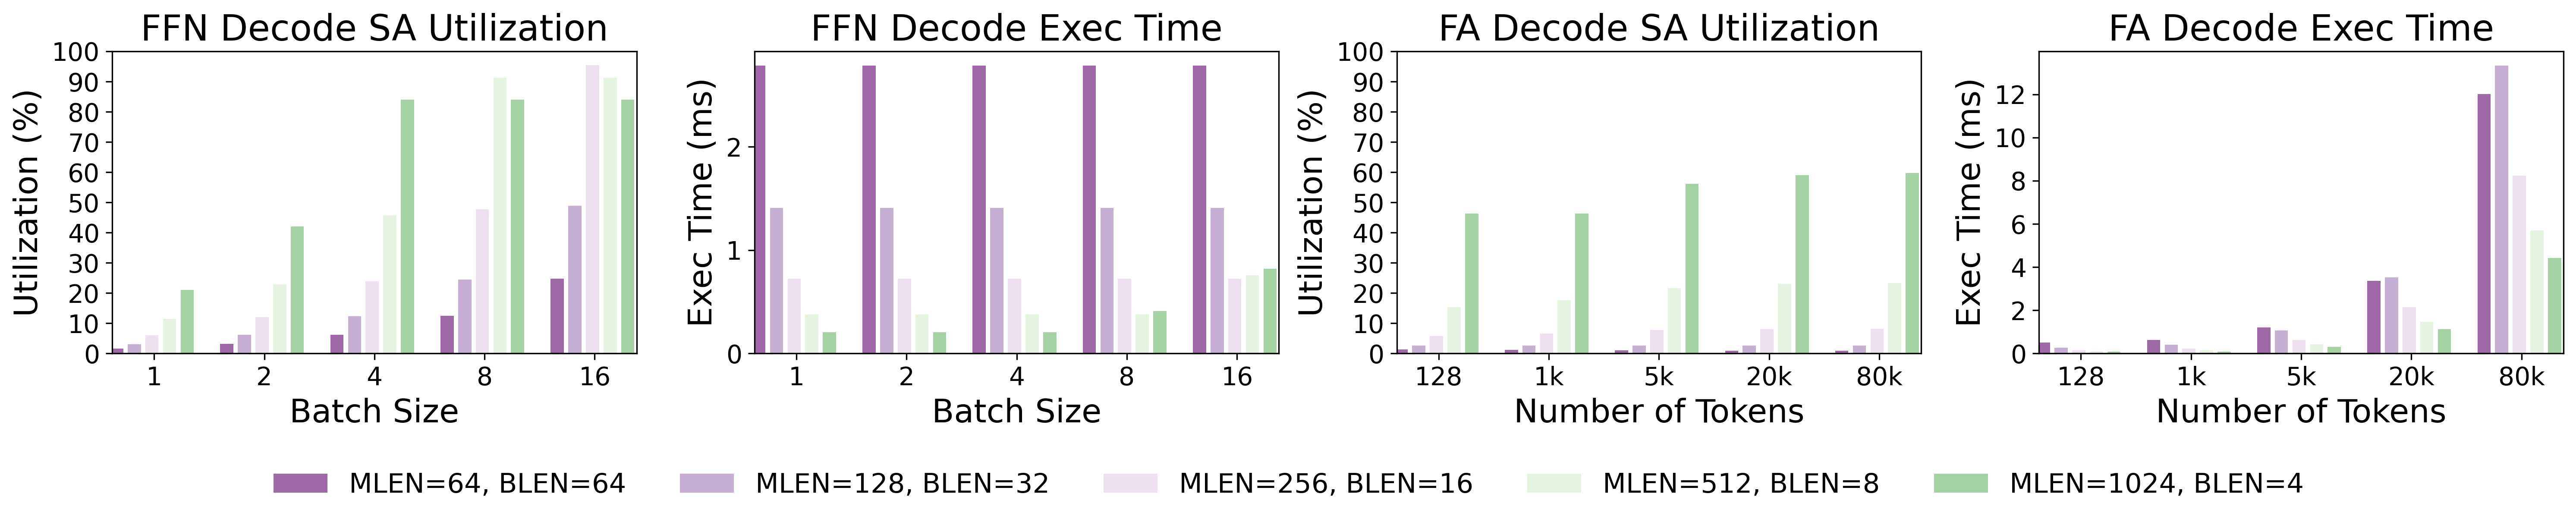
\includegraphics[width=1\textwidth]{Figures/Experiment/combined_FFN_FA_Utilization.png}
\caption{The systolic array reaches optimal utilization in the FFN layer when its block length (\texttt{BLEN}) aligns with the batch size.  
FA  = Flash Attention. SA = systolic array.
For FA, flattening the array enhances utilization by allowing parallel processing of multiple attention heads, and is particularly efficient for long-context inference with smaller effective batch sizes.}
  \label{tab:decode_FFN_SA}
\vspace{-10pt}
\end{figure*}

\begin{figure*}[t]
  \centering
  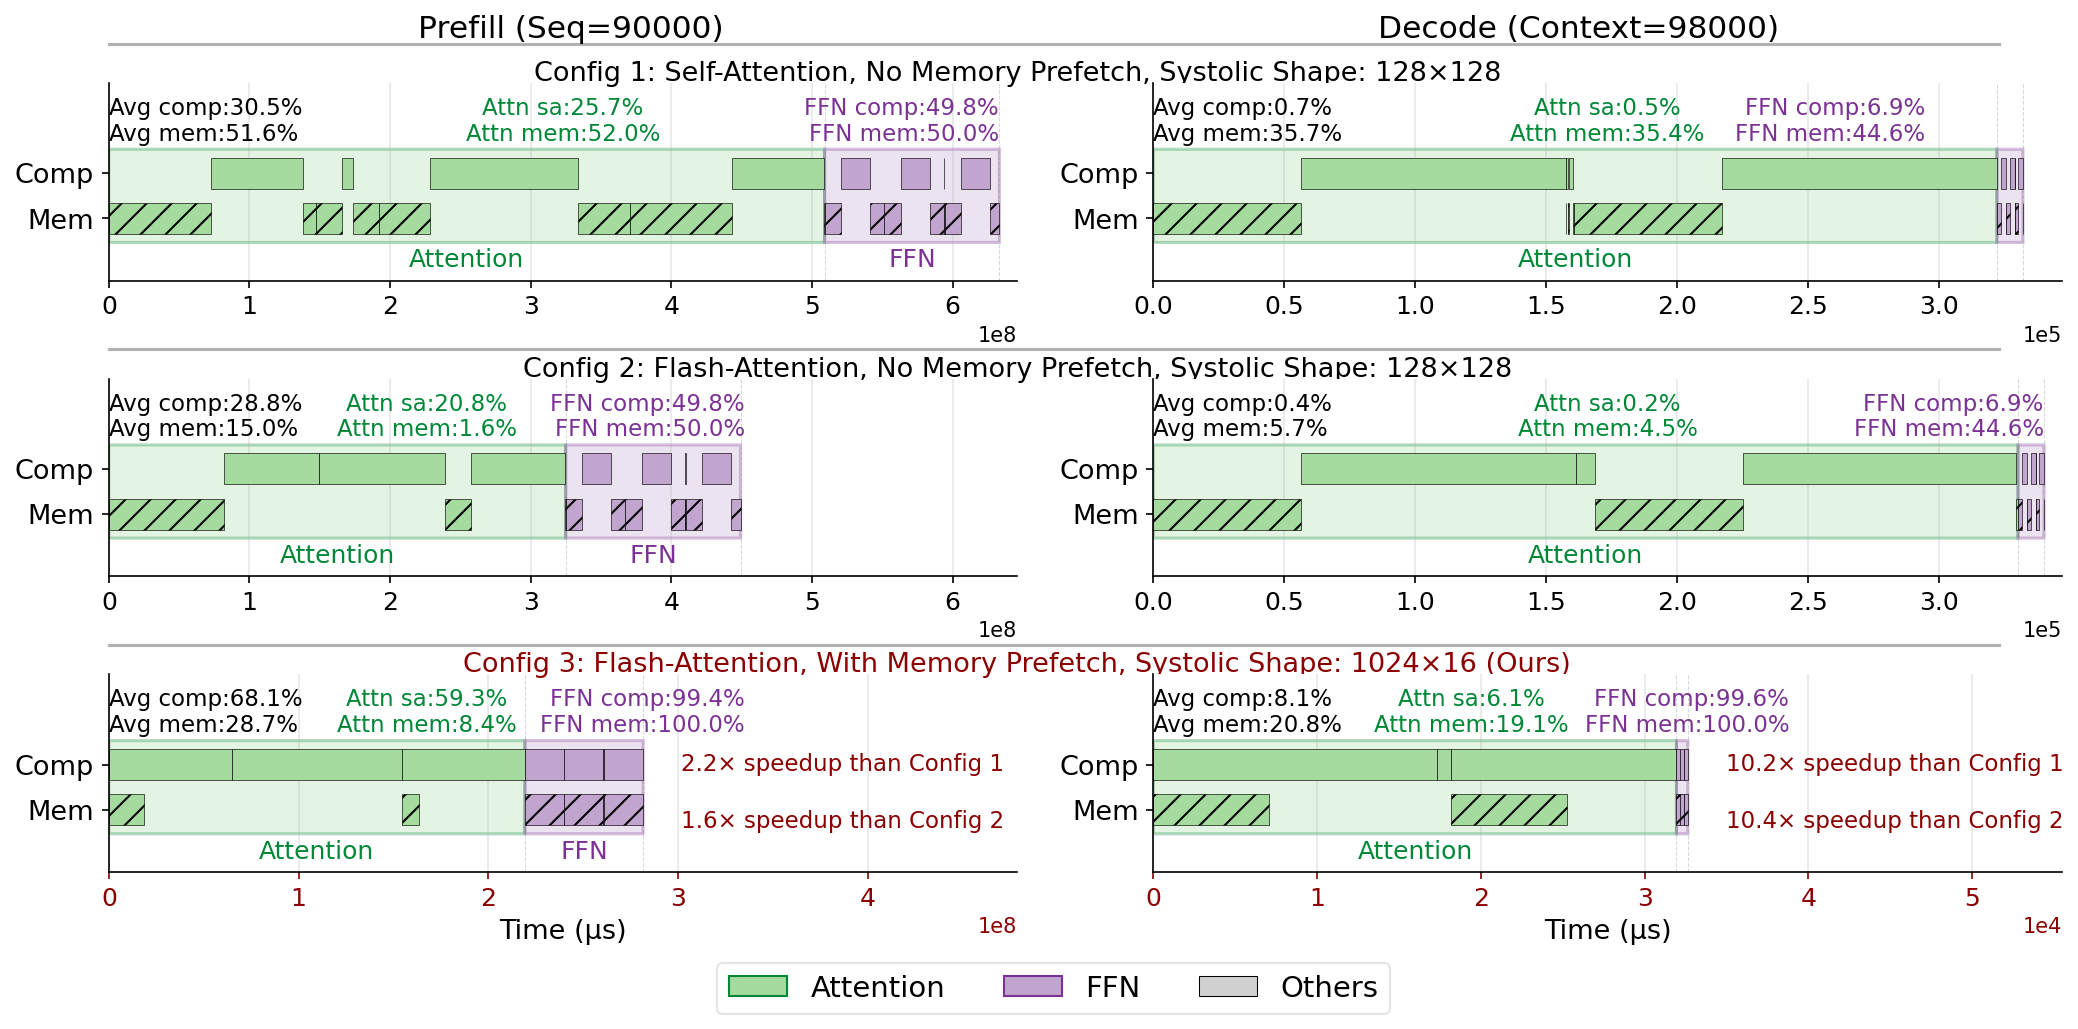
\includegraphics[width=1\textwidth]{Figures/Experiment/three_panel_timeline.png}
  \caption{This figure shows the timing performance breakdown of PLENA across the prefill and decode stages for the \llamaIIIPLUSBIG model with a batch size of 16. The breakdown includes compute active time (Comp), memory active time (Mem), systolic array (SA) utilization, and memory bandwidth utilization across the overall inference flow. With on-chip FlashAttention support, large intermediate activations are retained on-chip rather than written to off-chip memory, substantially reducing memory traffic, while memory prefetching hides most data-access latency. In addition, the flattened systolic array configuration maintains high utilization across both prefill and decode stages. For attention workloads, the flattened array achieves high compute and memory utilization by enabling parallel multi-head execution and head preloading.}
  \label{fig:hardware_ablation_study}
  \vspace{-5pt}
\end{figure*}






\paragraph{Abalation Study}

To further assess the impact of our key contributions, we conduct an ablation study on \llamaIIISmall to validate the effectiveness of 1) Output-norm guided blockwise clipping search and 2) Selective rotation. The ablation is structured into three stages: (i) \emph{weight-only} quantization, (ii) \emph{activation \& KV-cache} quantization on top of quantized weights, and (iii) \emph{full-system} emulation where all MX-aware operators are quantized. We show them in \Cref{tab:ablation}. 

First, MXFP4 always underperforms MXINT4 in all settings. Motivated by this, we adopt MXINT as the default data type for all subsequent evaluations. 
Second, for weight-only quantization, we show that rotation generally hurts performance -- they are simply not compatible with microscaling arithmetic. Furthermore, we demonstrate that our output-norm guided block-wise clipping ($\mathrm{Err}_{y}$) achieves better performance compared to weight-error guided block-wise clipping ($\mathrm{Err}_{w}$). 
Third, selective rotation effectively enhances activation and KV quantization for both MXFP4 and MXINT4. This is different from our observations with weight quantization, where rotation negatively impacts perplexity. We hypothesize this arises from the broader numerical range found in activation and KV values, which benefits from rotation's ability to temper the presence of outliers.
Finally, our full-system results confirm that both \emph{block-wise clipping search} and \emph{selective activation rotation} improve the overall performance.

\begin{table}[t]
\centering
\caption{Impact of quantization configurations on memory footprint and bandwidth
for \llamaIIIPLUSBIG under the OSWorld-L workload (90k prefill, 8k output tokens) in \Cref{tab:benchmark_token_usage} with batch size $B=8$.
W/A/KV denote the bit precision of weights, activations, and KV cache, respectively.}
\label{tab:quantization_levels}
\setlength{\tabcolsep}{5pt}
\renewcommand{\arraystretch}{1.05}
\begin{tabular}{lcccc}
\toprule
\textbf{W/A/KV (bits)} & 16/16/16 & 4/16/16 & 4/4/16 & 4/4/4 \\
\midrule
Peak Bandwidth (GB/s) & 8192 & 8192 & 5120 & 2048 \\
KV Cache Footprint (GB) & 239.26 & 239.26 & 239.26 & 59.81 \\
Weight Storage (GB) & 129.46 & 32.36 & 32.36 & 32.36 \\
\bottomrule
\end{tabular}
\vspace{-5pt}
\end{table}

%-----------------------------------
\subsection{Improving Utilization via Flattened Systolic Arrays}

The utilization analysis of PLENA’s flattened systolic array for the FFN and FlashAttention (FA) layers of the \llamaIIISmall model is summarized in \Cref{tab:decode_FFN_SA}. Results for the prefilling stage are omitted because both FFN and FA operate at near-maximum utilization during this phase. For FlashAttention, the computation pattern is independent of batch size, so it is not included in this table. For FFN, the computation for FFN is less important with the growth of generated token length, hence not included as well.



The DC synthesis results are reported in \Cref{tab:sa_hardware_comparison}. These results show that the flattened systolic array achieves higher compute-resource utilization for both the FFN and FlashAttention layers compared with prior accelerators. Furthermore, \Cref{fig:systolic_shape_comparison} demonstrates that the flattened systolic organization provides higher energy efficiency, despite some power and area overhead compared with conventional square arrays.

The overall ablation study of the systolic-array optimizations is presented in \Cref{fig:hardware_ablation_study}. The results show that the flattened systolic array, combined with native FlashAttention support, significantly reduces the execution time of both attention and FFN components across the prefill and decode phases, particularly for long-context inference.



\begin{table}[t]
  \centering
  \caption{Compute area, utilization, and attainable FLOPs for systolic arrays. 
    Baselines use \(64\times64\); PLENA uses \(4\times1024\). 
    \emph{S.A = Standard Attainable FLOPs in GSM8K (1.4k/200); A.A = Agentic Attainable FLOPs in OSWorld-L workload (90k/8k) in \Cref{tab:benchmark_token_usage}}}
  \label{tab:sa_hardware_comparison}
  
  \resizebox{1\linewidth}{!}{
  \begin{tabular}{lcccc}
    \toprule
    Metric & MicroscopiQ~\cite{Microscopiq} & Olive~\cite{guo2023olive} & FIGNA~\cite{FIGNA} & \textbf{PLENA} \\
    \midrule
    Comp Area (\(\mathrm{mm}^2\))   & 0.1378 & 0.319  & 0.471  & 0.237 \\
    TOPs/\(\mathrm{mm}^2\)          & 59.45  & 25.66  & 17.39  & 34.49 \\
    S.A FLOPs/\(\mathrm{mm}^2\)$^*$ & 3.36  & 1.60  & 7.51   & \best{29.31} \\
    A.A FLOPs/\(\mathrm{mm}^2\)$^*$ & 1.08   & 0.40   & 6.71   & \best{12.81} \\
    \bottomrule
  \end{tabular}
  }
  \vspace{-15pt}
\end{table}


\begin{figure}[!t]
  \centering
  \label{fig:systolic_shape_comparison}
  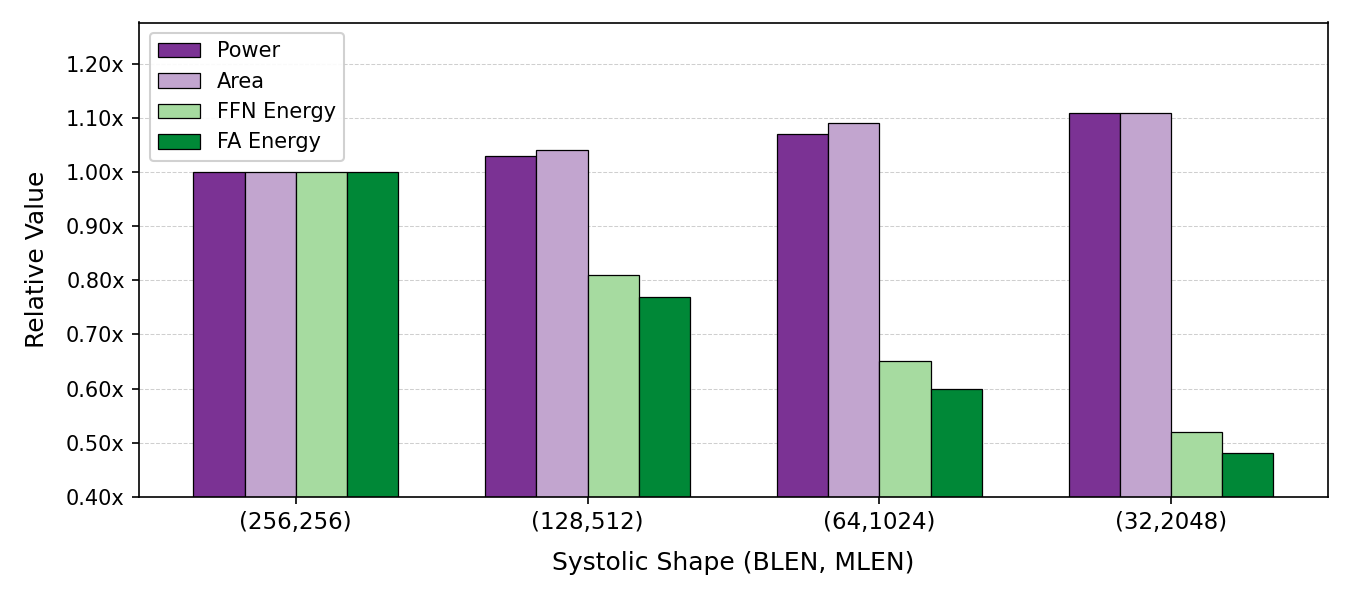
\includegraphics[width=0.485\textwidth]{Figures/systolic_shape_comparison.png}
    \caption{Power and area comparison of matrix units with different systolic array shapes. Although the flattened systolic array incurs slightly higher area and power, its higher utilization leads to significantly lower effective energy consumption for FFN and attention workloads in the agentic task OSWorld-L.}
    \vspace{-10pt}
\end{figure}



\begin{table*}[t]
  \centering
  \captionsetup{skip=2pt}
  \caption{System-level comparison across workloads in \Cref{tab:benchmark_token_usage}. Performance evaluation occurs under full HBM-capacity utilization, setting the batch size (BS) to the largest fitting value per workload-hardware pair. Note: We reproduced MicroScopiQ~\cite{Microscopiq} and deployed its compute unit on the PLENA platform for testing. And for GPT-OSS 20B (MoE)~\cite{MoE} and Qwen3-32B~\cite{qwen3}, the remaining accelerators and TPUs are not included since they do not support these configurations~\cite{vllm_tpu_supported_models}.}
  \label{tab:system_level_combined_reformat}
  \setlength{\tabcolsep}{3pt}
  \renewcommand{\arraystretch}{0.9}
  \scriptsize
  \begin{tabular}{lcccccccccccccccc}
    \toprule

% ==========================================================
% Model 1
% ==========================================================
\multicolumn{17}{c}{\textbf{\llamaIIIOneSMALL}} \\
\addlinespace[2pt]
& \multicolumn{4}{c}{\textbf{(1.4k, 0.2k)}}
& \multicolumn{4}{c}{\textbf{(114k, 5k)}}
& \multicolumn{4}{c}{\textbf{(90k, 8k)}}
& \multicolumn{4}{c}{\textbf{(90k, 8k) Equal Batch}} \\
\cmidrule(lr){2-5}\cmidrule(lr){6-9}\cmidrule(lr){10-13}\cmidrule(lr){14-17}
\textbf{System}
& TTFT (s) & TPS (×A100) & Tok/J & BS
& TTFT (s) & TPS (×A100) & Tok/J & BS
& TTFT (s) & TPS (×A100) & Tok/J & BS
& TTFT (s) & TPS (×A100) & Tok/J & BS \\
\midrule
A100
  & 0.68 & 1.00x  & 1.00x  & 2048
  & 7.40 & 1.00x  & 1.00x  & 16
  & 5.00 & 1.00x  & 1.00x  & 16
  & 5.00 & 1.00x  & 1.00x  & 16 \\
A100 QuaRot~\cite{QuaRot}
  & 0.73 & 1.12x & 1.12x & 4096
  & 8.63 & 1.10x & 1.10x & 32
  & 5.97 & 1.14x & 1.14x & 32
  & 4.79 & 1.08x & 1.08x & 16 \\
H100
  & 2.42 & 1.65x & 0.94x & 2048
  & 2.66 & 2.50x & 1.43x & 16
  & 1.83 & 2.48x & 1.41x & 16
  & 1.83 & 2.48x & 1.41x & 16\\
H100 QuaRot~\cite{QuaRot}
  & 2.51 & 1.77x & 1.01x & 4096
  & 2.97 & 2.57x & 1.47x & 32
  & 2.01 & 2.55x & 1.46x & 32
  & 1.77 & 2.51x & 1.43x & 16 \\
TPU v6e
  & 5.61 & 0.88x & N/A & 2048
  & 7.58 & 0.51x & N/A & 16
  & 7.23 & 0.53x & N/A & 16
  & 7.23 & 0.53x & N/A & 16 \\
MicroScopiQ~\cite{Microscopiq}
  & 3.47 & 0.83x & 1.67x & 8192
  & 21.28 & 0.37x & 0.74x & 64
  & 19.13 & 0.39x & 0.78x & 64
  & 4.93 & 0.27x & 0.54x & 16 \\ 
\textbf{PLENA}
  & 3.41 & \best{1.91x} & \best{3.50x} & 8192
  & 20.13 & 1.45x & \best{2.66x} & 64
  & 18.87 & 1.45x & \best{2.65x} & 64
  & 4.68 & 1.17x & \best{2.10x} & 16 \\
\midrule

% ==========================================================
% Model 2
% ==========================================================
\multicolumn{17}{c}{\textbf{\llamaIIIPLUSBIG}} \\
\addlinespace[2pt]
& \multicolumn{4}{c}{\textbf{(1.4k, 0.2k)}}
& \multicolumn{4}{c}{\textbf{(114k, 5k)}}
& \multicolumn{4}{c}{\textbf{(90k, 8k)}}
& \multicolumn{4}{c}{\textbf{(90k, 8k) Equal Batch}} \\
\cmidrule(lr){2-5}\cmidrule(lr){6-9}\cmidrule(lr){10-13}\cmidrule(lr){14-17}
\textbf{System}
& TTFT (s) & TPS (×A100) & Tok/J & BS
& TTFT (s) & TPS (×A100) & Tok/J & BS
& TTFT (s) & TPS (×A100) & Tok/J & BS
& TTFT (s) & TPS (×A100) & Tok/J & BS \\
\midrule
A100
  & 0.78  & 1.00x  & 1.00x & 256
  & 43.18 & 1.00x  & 1.00x  & 4
  & 29.67 & 1.00x  & 1.00x  & 4
  & 29.67 & 1.00x  & 1.00x  & 4 \\
A100 QuaRot~\cite{QuaRot}
  & 1.17 & 1.08x & 1.08x & 512
  & 42.89 & 1.13x & 1.13x & 8
  & 32.17 & 1.13x & 1.13x & 8
  & 27.69 & 1.11x & 1.11x & 4 \\
H100
  & 0.34 & 2.34x & 1.34x & 256
  & 14.30 & 2.13x & 1.21x & 4
  & 10.10 & 2.04x & 1.22x & 4
  & 10.10 & 2.04x & 1.22x & 4 \\
H100 QuaRot~\cite{QuaRot}
  & 0.44 & 2.36x & 1.35x & 512
  & 16.12 & 2.19x & 1.25x & 8
  & 11.37 & 2.14x & 1.22x & 8
  & 9.88 & 2.08x & 1.18x & 4 \\
TPU v6e
  & 11.7 & 0.85x & N/A & 256
  & 41.96 & 0.46x & N/A & 4
  & 37.61 & 0.47x & N/A & 4
  & 37.61 & 0.47x & N/A & 4 \\
MicroScopiQ~\cite{Microscopiq}
  & 8.32 & 0.79 & 1.59x & 1024
  & 73.28 & 0.20x & 0.41x & 16
  & 49 & 0.17x & 0.35x & 16
  & 23.93 & 0.11x & 0.23x & 4 \\
\textbf{PLENA}
  & 7.58 & 1.82x & \best{3.32x} & 1024
  & 69.10 & \best{2.23x} & \best{4.07x} & 16
  & 43.43 & \best{2.21x} & \best{4.04x} & 16
  & 21.68 & 1.34x & \best{2.45x} & 4\\
\midrule

% ==========================================================
% Model 3
% ==========================================================
\multicolumn{17}{c}{\textbf{GPT-OSS 20B (MoE)}} \\
\addlinespace[2pt]
& \multicolumn{4}{c}{\textbf{(1.4k, 0.2k)}}
& \multicolumn{4}{c}{\textbf{(114k, 5k)}}
& \multicolumn{4}{c}{\textbf{(90k, 8k)}}
& \multicolumn{4}{c}{\textbf{(90k, 8k) Equal Batch}} \\
\cmidrule(lr){2-5}\cmidrule(lr){6-9}\cmidrule(lr){10-13}\cmidrule(lr){14-17}
\textbf{System}
& TTFT (s) & TPS (×A100) & Tok/J & BS
& TTFT (s) & TPS (×A100) & Tok/J & BS
& TTFT (s) & TPS (×A100) & Tok/J & BS
& TTFT (s) & TPS (×A100) & Tok/J & BS \\
\midrule
A100
  & 1.46 & 1.00x  & 1.00x  & 1024
  & 11.81 & 1.00x  & 1.00x  & 8
  & 8.05 & 1.00x  &  1.00x & 8
  & 8.05 & 1.00x  & 1.00x  & 8 \\
H100
  & 4.03 & 0.89x  & 0.51x & 1024
  & 1.85 & 3.10x & 1.78x & 8
  & 1.38 & 2.90x & 1.66x & 8
  & 1.38 & 2.90x & 1.66x & 8\\
\textbf{PLENA}
  & 13.41 & \best{1.15x} & \best{2.10x} & 4096
  & 47.63 & 1.96x & \best{3.58x} & 64
  & 41.08 & 1.93x & \best{3.52x} & 64
  & 9.77 & 0.99x & \best{1.79x} & 8 \\
\midrule

% ==========================================================
% Model 4
% ==========================================================
\multicolumn{17}{c}{\textbf{Qwen3-32B}} \\
\addlinespace[2pt]
& \multicolumn{4}{c}{\textbf{(1.4k, 0.2k)}}
& \multicolumn{4}{c}{\textbf{(114k, 5k)}}
& \multicolumn{4}{c}{\textbf{(90k, 8k)}}
& \multicolumn{4}{c}{\textbf{(90k, 8k) Equal Batch}} \\
\cmidrule(lr){2-5}\cmidrule(lr){6-9}\cmidrule(lr){10-13}\cmidrule(lr){14-17}
\textbf{System}
& TTFT (s) & TPS (×A100) & Tok/J & BS
& TTFT (s) & TPS (×A100) & Tok/J & BS
& TTFT (s) & TPS (×A100) & Tok/J & BS
& TTFT (s) & TPS (×A100) & Tok/J & BS \\
\midrule
A100
  & 0.88 & 1.00x & 1.00x  & 1024
  & 28.90 & 1.00x  & 1.00x  & 8
  & 19.19 & 1.00x  & 1.00x  & 8
  & 19.19 & 1.00x  & 1.00x  & 8 \\
H100
  & 1.19 & 2.13x & 1.22x & 1024
  & 9.24 & 2.29x & 1.31x & 8
  & 6.29 & 2.21x & 1.26x & 8 
  & 6.29 & 2.21x & 1.26x & 8  \\
\textbf{PLENA}
  & 4.38 & 1.40x & \best{2.56x} & 4096
  & 108.1 & 1.22x & \best{2.23x} & 64
  & 90.71 & 1.23x & \best{2.25x} & 64
  & 23.14 & 1.14x & \best{2.08x} & 8 \\
\bottomrule
  \end{tabular}
  % \vspace{-8pt}
\end{table*}

%-----------------------------------
\subsection{System Performance Analysis}

\begin{table}[t]
\centering
\caption{Token usage (prefill/output) across benchmarks:
GSM8K~\cite{gsm8k},
BFCL-Web Search Base~\cite{bfcl},
OSWorld LibreOffice (OSWorld-L)~\cite{osworld}.}
\label{tab:benchmark_token_usage}
\setlength{\tabcolsep}{3pt}
\renewcommand{\arraystretch}{0.9}
\small
\begin{tabular}{lccc}
\toprule
 & GSM8K & BFCL-W & OSWorld-L  \\
\midrule
Prefill (Tokens) & 1.4k & 114k & 90k  \\
Output (Tokens) & 0.2k & 5k   & 8k  \\
\bottomrule
\end{tabular}
\vspace{-10pt}
\end{table}

The system-level performance comparison is shown in \Cref{tab:system_level_combined_reformat}, evaluating both small and large GQA-based LLaMA models as well as the recently published MoE-based GPT-OSS model and Qwen3-32B and supporting long-context inputs. The performance results for PLENA and MicroScopiQ are obtained using our transactional simulator, modeling performance in a 7 nm technology node. For fairness, we conduct a system-level comparison against a 4$\times$A100 SXM GPU system (80\,GB HBM and 1.99\,TB/s bandwidth per GPU), a 4$\times$H100 SXM GPU system (80\,GB HBM and 3.35\,TB/s bandwidth per GPU), and a 16$\times$TPU v6e system (32\,GB HBM and 1.56\,TB/s bandwidth per device). Both PLENA and MicroScopiQ are modeled as 16-accelerator systems with aggregate HBM capacity and bandwidth equivalent to the TPU system. To account for GPUs' non-compute components, the number of devices is determined by approximately aligning multiplier counts rather than silicon area. The co-design-selected PLENA configuration—(\texttt{BLEN} = 32, \texttt{MLEN} = 2048, \texttt{VLEN} = 2048, Precision W/A/KV = 4/4/4)—demonstrates improved performance across all evaluated workloads.

As shown, PLENA achieves higher TPS than both the A100 and TPU v6e under identical HBM settings and multiplier counts, reaching up to 2.23$\times$that of the A100 and 4.70$\times$ that of the TPU v6e for agentic workload. The higher TTFT observed in PLENA is explained by its ability to store more batches within the same HBM capacity using our quantization scheme. As batch size increases, the prefill stage grows longer due to additional memory accesses and computation.
